\documentclass[11pt,a4paper]{article}

% ------------------------------------------------------------------
% Packages
% ------------------------------------------------------------------
\usepackage[T1]{fontenc}
\usepackage[utf8]{inputenc}
\usepackage{lmodern}
\usepackage[english]{babel}
\usepackage[a4paper,margin=2.3cm,headheight=14pt]{geometry}
\usepackage{microtype}
\usepackage{graphicx}
\usepackage{float}
\usepackage{caption}
\usepackage{subcaption}
\usepackage{booktabs}
\usepackage{array}
\usepackage{tabularx}
\usepackage{makecell}
\usepackage{enumitem}
\usepackage{siunitx}
\usepackage{xcolor}
\usepackage{listings}
\usepackage[most]{tcolorbox}
\usepackage{fancyhdr}
\usepackage{titlesec}
\usepackage{tikz}
\usetikzlibrary{arrows.meta,positioning,shapes.geometric,shapes.misc,calc,fit,backgrounds,shadows}
\usepackage{pgfplots}
\pgfplotsset{compat=1.17}
\usepackage[hidelinks]{hyperref}

% ------------------------------------------------------------------
% Colours and styles
% ------------------------------------------------------------------
\definecolor{navy}{HTML}{0B3D5C}
\definecolor{sky}{HTML}{0A84C6}
\definecolor{coolblue}{HTML}{2F9BFF}
\definecolor{heatred}{HTML}{EA4D4D}
\definecolor{okgreen}{HTML}{3FBF6F}
\definecolor{amber}{HTML}{FFB020}
\definecolor{nrred}{HTML}{8F0000}
\definecolor{codebg}{HTML}{F6F8FA}
\definecolor{codegray}{HTML}{6A737D}

\captionsetup{font=small,labelfont={bf,color=navy},format=hang}
\setlist{itemsep=2pt,topsep=4pt}

\titleformat{\section}{\Large\bfseries\color{navy}}{\thesection}{0.8em}{}
\titleformat{\subsection}{\large\bfseries\color{navy!85}}{\thesubsection}{0.8em}{}
\titleformat{\subsubsection}{\normalsize\bfseries\color{navy!75}}{\thesubsubsection}{0.8em}{}

\pagestyle{fancy}
\fancyhf{}
\fancyhead[L]{\small\color{codegray}Smart Air Conditioner: ESP32, DHT11, MQTT, Node-RED}
\fancyhead[R]{\small\color{codegray}IoT course, ENP}
\fancyfoot[C]{\small\thepage}
\renewcommand{\headrulewidth}{0.4pt}

\lstdefinestyle{cpp}{
  language=C++, basicstyle=\ttfamily\footnotesize, backgroundcolor=\color{codebg},
  keywordstyle=\color{sky}\bfseries, commentstyle=\color{codegray}\itshape,
  stringstyle=\color{heatred!80!black}, numbers=left, numberstyle=\tiny\color{codegray},
  frame=single, rulecolor=\color{black!12}, breaklines=true, showstringspaces=false,
  tabsize=2, xleftmargin=1.6em, framexleftmargin=1.4em, columns=fullflexible,
  morekeywords={String,byte,uint32_t}, literate={°}{{\textdegree}}1
}
\lstdefinestyle{js}{
  style=cpp, language=Java, morekeywords={const,let,return,null,typeof},
  literate={°}{{\textdegree}}1
}
\lstdefinestyle{json}{
  basicstyle=\ttfamily\footnotesize, backgroundcolor=\color{codebg}, frame=single,
  rulecolor=\color{black!12}, breaklines=true, columns=fullflexible
}

\newtcolorbox{keybox}[1][]{colback=sky!6,colframe=sky,boxrule=0.6pt,arc=2pt,
  left=6pt,right=6pt,top=4pt,bottom=4pt,fonttitle=\bfseries\small,title=#1}

\newcommand{\topic}[1]{\texttt{\small #1}}
\newcommand{\shot}[2][\linewidth]{\includegraphics[width=#1]{#2}}

% TikZ styles
\tikzset{
  blk/.style={draw=navy,thick,rounded corners=3pt,fill=white,align=center,
              minimum height=1.1cm,font=\small,drop shadow={opacity=0.15}},
  layer/.style={draw=none,rounded corners=6pt,inner sep=8pt},
  arr/.style={-{Stealth[length=2.6mm]},thick},
  darr/.style={{Stealth[length=2.6mm]}-{Stealth[length=2.6mm]},thick},
  lbl/.style={font=\scriptsize,fill=white,inner sep=1.5pt,align=center},
}

% ------------------------------------------------------------------
\begin{document}
% ------------------------------------------------------------------

% ======================= TITLE PAGE ===============================
\begin{titlepage}
\thispagestyle{empty}
\centering
{\large\textsc{People's Democratic Republic of Algeria}\par}
\vspace{2pt}
{\normalsize Ministry of Higher Education and Scientific Research\par}
\vspace{14pt}
{\LARGE\bfseries\color{navy} École Nationale Polytechnique\par}
\vspace{4pt}
{\large Industrial Engineering Department, Data Science and AI option\par}
\vspace{1.6cm}

{\color{sky}\rule{\linewidth}{1.2pt}}\par\vspace{10pt}
{\large Internet of Things (IoT) course, homework report\par}
\vspace{10pt}
{\Huge\bfseries\color{navy} Smart Air Conditioner\par}
\vspace{8pt}
{\Large ESP32 + DHT11 sensor, MQTT protocol\\[2pt] and Node-RED dashboard, simulated on Wokwi\par}
\vspace{8pt}
{\color{sky}\rule{\linewidth}{1.2pt}}\par
\vspace{1.2cm}

% ---- cover illustration --------------------------------------------
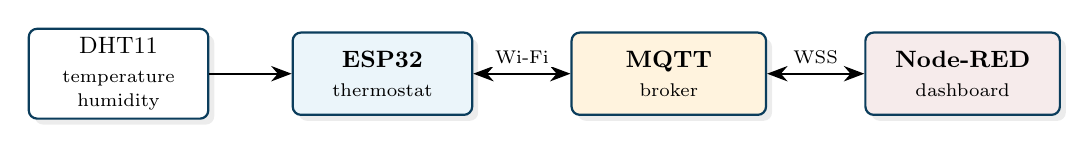
\begin{tikzpicture}[scale=0.95,every node/.style={transform shape}]
  \node[blk,minimum width=2.4cm] (s) {DHT11\\\scriptsize temperature\\[-2pt]\scriptsize humidity};
  \node[blk,right=1.1cm of s,minimum width=2.4cm,fill=sky!8] (e) {\textbf{ESP32}\\\scriptsize thermostat};
  \node[blk,right=1.3cm of e,minimum width=2.6cm,fill=amber!15] (b) {\textbf{MQTT}\\\scriptsize broker};
  \node[blk,right=1.3cm of b,minimum width=2.6cm,fill=nrred!8] (n) {\textbf{Node-RED}\\\scriptsize dashboard};
  \draw[arr] (s) -- (e);
  \draw[darr] (e) -- node[lbl,above=2pt]{Wi-Fi} (b);
  \draw[darr] (b) -- node[lbl,above=2pt]{WSS} (n);
\end{tikzpicture}

\vfill
\begin{tabular}{rl}
  \textbf{Student:} & Ahcene Zakaria \textsc{Aouanouk} \\
  \textbf{Programme:} & Industrial Engineering, Data Science and AI (class of 2027)\\
  \textbf{Tools:} & Wokwi, Arduino (C++), MQTT, Node-RED, FlowFuse Dashboard 2.0\\
  \textbf{Online project:} & \url{https://wokwi.com/projects/481300995020006401}\\
\end{tabular}

\vspace{1.2cm}
{\large Academic year 2026--2027 \quad$\cdot$\quad November 2026\par}
\end{titlepage}

% ======================= ABSTRACT + TOC ===========================
\begin{abstract}
\noindent This report presents the design, implementation and testing of a connected air
conditioner prototype. An ESP32 micro-controller reads the room temperature and humidity
from a DHT11 sensor, runs a thermostat with hysteresis that drives a cooling stage, a heating
stage and a variable-speed swinging louver, and displays its state on a local LCD. The device
publishes its telemetry over the MQTT protocol and accepts remote commands (power, mode,
setpoint). A Node-RED flow subscribes to the telemetry and exposes a web dashboard with
gauges, a history chart, status indicators, alerts and remote controls. The whole system was
simulated on Wokwi and tested end to end with a real public MQTT broker and a Node-RED
server running on a Windows laptop. All the scenarios (cooling, heating, fan only, power off,
setpoint change, device disconnection) behaved as specified.
\end{abstract}

\tableofcontents
\listoffigures
\newpage

% ======================= 1. INTRODUCTION ==========================
\section{Introduction}

Air conditioners are among the most common appliances that benefit from the Internet of
Things: a connected unit can be monitored and controlled remotely, can report its state and
can react automatically to the measured temperature. The goal of this homework is to build
such a system with three imposed technologies:

\begin{itemize}
  \item an \textbf{ESP32} board with a \textbf{DHT11} temperature and humidity sensor,
        simulated on \textbf{Wokwi};
  \item the \textbf{MQTT} protocol to exchange data between the device and the application;
  \item \textbf{Node-RED} to build the monitoring and control \textbf{dashboard}.
\end{itemize}

\subsection{Objectives}
\begin{enumerate}
  \item Measure the room temperature and humidity periodically.
  \item Implement the air-conditioning logic: automatic cooling or heating to reach a
        setpoint, with a hysteresis band to protect the compressor.
  \item Publish the device state (telemetry) to an MQTT broker.
  \item Control the unit remotely (ON/OFF, mode, setpoint) from a dashboard.
  \item Detect when the device goes offline and raise an alert when the room overheats.
\end{enumerate}

\subsection{Deliverables}
\begin{itemize}
  \item The Wokwi project, made of three files: the circuit \texttt{diagram.json}, the
        firmware \texttt{sketch.ino} and the library list \texttt{libraries.txt}.
  \item The Node-RED flow (\texttt{flows.json}) and its dashboard.
  \item This report, with the design choices, the implementation and the test results.
\end{itemize}

% ======================= 2. BACKGROUND ============================
\section{Background}

\subsection{Layered IoT architecture}
An IoT system is usually described with three layers (Figure~\ref{fig:layers}):
\begin{itemize}
  \item \textbf{Perception layer}: sensors and actuators that interact with the physical world
        (here the DHT11, LEDs, servo motor, buzzer, LCD and push button).
  \item \textbf{Network layer}: transports the data (Wi-Fi, TCP/IP, MQTT and the broker).
  \item \textbf{Application layer}: processes, stores and presents the data to the user
        (Node-RED and its dashboard).
\end{itemize}

\begin{figure}[H]
\centering
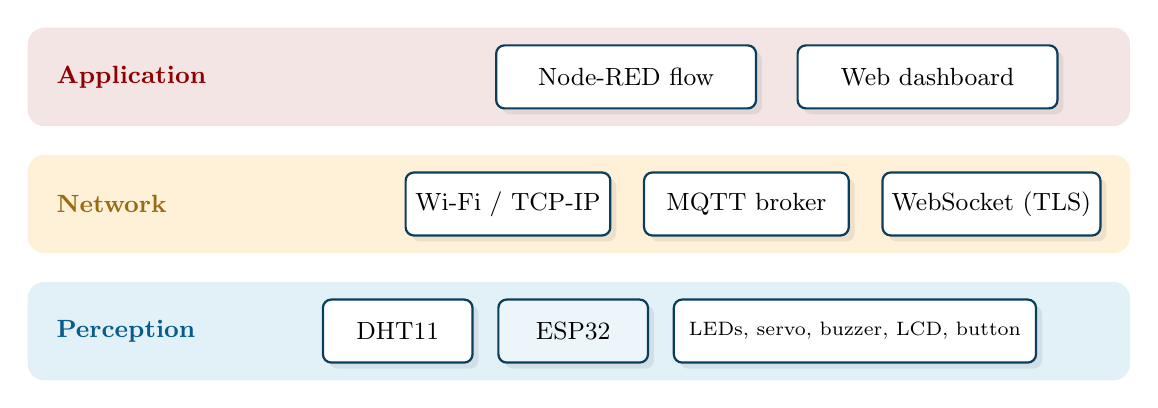
\begin{tikzpicture}[node distance=0.35cm]
  \node[layer,fill=nrred!10,minimum width=14cm,minimum height=1.25cm] (app) {};
  \node[anchor=west,font=\bfseries\small,color=nrred] at ($(app.west)+(0.25,0)$) {Application};
  \node[blk,minimum width=3.3cm,minimum height=0.8cm] at ($(app.center)+(0.6,0)$) (nr) {Node-RED flow};
  \node[blk,minimum width=3.3cm,minimum height=0.8cm,right=0.5cm of nr] (db) {Web dashboard};

  \node[layer,fill=amber!18,minimum width=14cm,minimum height=1.25cm,below=of app] (net) {};
  \node[anchor=west,font=\bfseries\small,color=amber!60!black] at ($(net.west)+(0.25,0)$) {Network};
  \node[blk,minimum width=2.6cm,minimum height=0.8cm] at ($(net.center)+(-0.9,0)$) (wifi) {Wi-Fi / TCP-IP};
  \node[blk,minimum width=2.6cm,minimum height=0.8cm,right=0.4cm of wifi] (mq) {MQTT broker};
  \node[blk,minimum width=2.6cm,minimum height=0.8cm,right=0.4cm of mq] (ws) {WebSocket (TLS)};

  \node[layer,fill=sky!12,minimum width=14cm,minimum height=1.25cm,below=of net] (per) {};
  \node[anchor=west,font=\bfseries\small,color=sky!70!black] at ($(per.west)+(0.25,0)$) {Perception};
  \node[blk,minimum width=1.9cm,minimum height=0.8cm] at ($(per.center)+(-2.3,0)$) (dht) {DHT11};
  \node[blk,minimum width=1.9cm,minimum height=0.8cm,right=0.3cm of dht,fill=sky!8] (esp) {ESP32};
  \node[blk,minimum width=4.6cm,minimum height=0.8cm,right=0.3cm of esp,font=\scriptsize] (act) {LEDs, servo, buzzer, LCD, button};
\end{tikzpicture}
\caption{Three-layer architecture of the smart air conditioner.}
\label{fig:layers}
\end{figure}

\subsection{The MQTT protocol}
MQTT (\emph{Message Queuing Telemetry Transport}) is a lightweight publish/subscribe protocol
designed for constrained devices and unreliable networks. It runs on top of TCP (default port
1883, 8883 with TLS) or on top of WebSockets.

\begin{itemize}
  \item \textbf{Broker}: central server that receives every message and forwards it to the
        clients that subscribed to its topic. Publishers and subscribers never talk directly,
        they are decoupled in space and time.
  \item \textbf{Topic}: hierarchical UTF-8 string such as \topic{enp/zaki/ac/telemetry}.
        Wildcards: \topic{+} matches one level, \topic{\#} matches all remaining levels.
  \item \textbf{QoS} (quality of service): 0 = at most once, 1 = at least once (acknowledged),
        2 = exactly once.
  \item \textbf{Retained message}: the broker stores the last message of a topic and delivers
        it immediately to every new subscriber.
  \item \textbf{Last Will and Testament (LWT)}: message registered by the client at connection
        time; the broker publishes it if the client disappears without a clean disconnection.
  \item \textbf{Keep-alive}: periodic ping that lets the broker detect dead clients.
\end{itemize}

\begin{keybox}[Why MQTT for this project]
The payloads are tiny (about 120 bytes), the device must both \emph{send} data and
\emph{receive} commands, and the dashboard must know when the device is offline. MQTT covers
the three needs natively with publish/subscribe, persistent bidirectional connections and the
Last Will mechanism, with a much smaller overhead than HTTP polling.
\end{keybox}

\subsection{Hardware and software}
\begin{description}[style=nextline,leftmargin=1.2em]
  \item[ESP32] Dual-core Xtensa LX6 micro-controller (up to \SI{240}{MHz}) with integrated
        Wi-Fi 802.11 b/g/n and Bluetooth. Programmed in C++ with the Arduino framework.
  \item[DHT11] Low-cost digital temperature and humidity sensor using a single-wire protocol.
        Range \SIrange{0}{50}{\celsius} (\SI{\pm 2}{\celsius}) and 20 to 90\,\% RH
        (\SI{\pm 5}{\percent}), at most one reading per second.
  \item[Wokwi] Online electronics simulator. It emulates the ESP32, its peripherals and Wi-Fi:
        the virtual access point \texttt{Wokwi-GUEST} gives the simulated board real Internet
        access, so it can reach a public MQTT broker.
  \item[Node-RED] Flow-based, low-code programming tool built on Node.js. Messages travel along
        wires between nodes (MQTT in/out, function, change, \dots). The FlowFuse
        \textbf{Dashboard 2.0} package adds web widgets (gauges, charts, switches, sliders).
\end{description}

% ======================= 3. SYSTEM DESIGN =========================
\section{System design}

\subsection{Global architecture}
Figure~\ref{fig:archi} shows the complete data path. The ESP32 publishes its telemetry to the
broker every two seconds; Node-RED subscribes to it and feeds the dashboard widgets. In the
opposite direction, every action on the dashboard is published on a command topic, the broker
forwards it to the ESP32 which applies it immediately.

\begin{figure}[H]
\centering
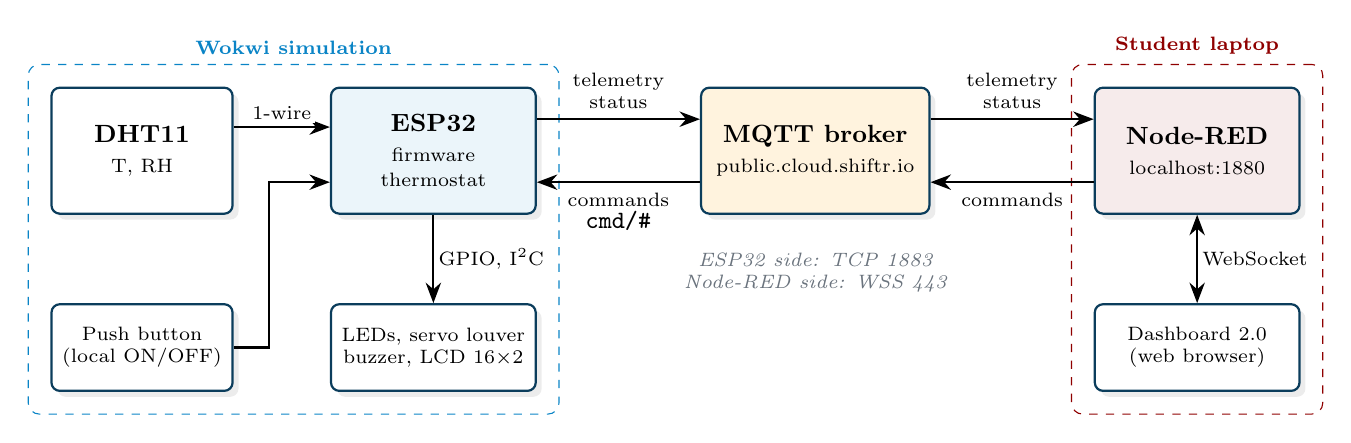
\begin{tikzpicture}
  \node[blk,minimum width=2.3cm,minimum height=1.6cm] (dht) at (0,0) {\textbf{DHT11}\\\scriptsize T, RH};
  \node[blk,minimum width=2.6cm,minimum height=1.6cm,fill=sky!8] (esp) at (3.7,0) {\textbf{ESP32}\\\scriptsize firmware\\[-2pt]\scriptsize thermostat};
  \node[blk,minimum width=2.6cm,font=\scriptsize] (act) at (3.7,-2.5) {LEDs, servo louver\\buzzer, LCD 16$\times$2};
  \node[blk,minimum width=2.3cm,font=\scriptsize] (btn) at (0,-2.5) {Push button\\(local ON/OFF)};
  \node[blk,minimum width=2.9cm,minimum height=1.6cm,fill=amber!15] (brk) at (8.55,0) {\textbf{MQTT broker}\\\scriptsize public.cloud.shiftr.io};
  \node[blk,minimum width=2.6cm,minimum height=1.6cm,fill=nrred!8] (nr) at (13.4,0) {\textbf{Node-RED}\\\scriptsize localhost:1880};
  \node[blk,minimum width=2.6cm,font=\scriptsize] (ui) at (13.4,-2.5) {Dashboard 2.0\\(web browser)};

  \draw[arr] ([yshift=3mm]dht.east) -- node[lbl,above=1pt]{1-wire} ([yshift=3mm]esp.west);
  \draw[arr] (btn.east) -- ++(0.45,0) |- ([yshift=-4mm]esp.west);
  \draw[arr] (esp) -- node[lbl,right]{GPIO, I\textsuperscript{2}C} (act);
  \draw[arr] ([yshift=4mm]esp.east) -- node[lbl,above=2pt]{telemetry\\status} ([yshift=4mm]brk.west);
  \draw[arr] ([yshift=-4mm]brk.west) -- node[lbl,below=2pt]{commands\\\topic{cmd/\#}} ([yshift=-4mm]esp.east);
  \draw[arr] ([yshift=4mm]brk.east) -- node[lbl,above=2pt]{telemetry\\status} ([yshift=4mm]nr.west);
  \draw[arr] ([yshift=-4mm]nr.west) -- node[lbl,below=2pt]{commands} ([yshift=-4mm]brk.east);
  \draw[darr] (nr) -- node[lbl,right]{WebSocket} (ui);
  \node[font=\scriptsize\itshape,color=codegray,align=center] at (8.55,-1.55) {ESP32 side: TCP 1883\\Node-RED side: WSS 443};
  \begin{scope}[on background layer]
    \node[draw=sky,dashed,rounded corners,fit=(dht)(esp)(act)(btn),inner sep=8pt,
          label={[font=\scriptsize\bfseries,color=sky]above:Wokwi simulation}] {};
    \node[draw=nrred,dashed,rounded corners,fit=(nr)(ui),inner sep=8pt,
          label={[font=\scriptsize\bfseries,color=nrred]above:Student laptop}] {};
  \end{scope}
\end{tikzpicture}

\caption{End-to-end architecture: telemetry path (top arrows) and command path (bottom arrows).}
\label{fig:archi}
\end{figure}

\subsection{Hardware components and wiring}

Table~\ref{tab:pins} lists the components and their connections. Each LED has a
\SI{220}{\ohm} series resistor. The push button uses the internal pull-up of the ESP32, so it
reads \texttt{LOW} when pressed.

\begin{table}[H]
\centering\small
\caption{Components, role and ESP32 pin mapping.}
\label{tab:pins}
\begin{tabularx}{\linewidth}{@{}l X l@{}}
\toprule
\textbf{Component} & \textbf{Role in the air conditioner} & \textbf{ESP32 pins} \\
\midrule
DHT11 (DHT22 part in Wokwi) & Room temperature and humidity & DATA $\to$ GPIO 32, VCC 3V3 \\
Blue LED + \SI{220}{\ohm} & Compressor in \textbf{cooling} mode & GPIO 26 \\
Red LED + \SI{220}{\ohm}  & \textbf{Heating} (heat pump) & GPIO 25 \\
Green LED + \SI{220}{\ohm} & Unit powered \textbf{ON} & GPIO 27 \\
Servo motor & Swinging air louver, speed = fan speed & PWM $\to$ GPIO 18, V+ 5V \\
Buzzer & Beep when a command is received & GPIO 19 \\
LCD 16$\times$2, I\textsuperscript{2}C (0x27) & Local display of T, RH, mode, state & SDA GPIO 21, SCL GPIO 22 \\
Push button & Local power ON/OFF & GPIO 4 (\texttt{INPUT\_PULLUP}) \\
\bottomrule
\end{tabularx}
\end{table}

\begin{keybox}[Note on the sensor]
Wokwi does not provide a DHT11 part. The DHT22 part is used instead: it speaks the same
single-wire protocol and is read with the same Adafruit \texttt{DHT} library. On the real board,
the only change is \texttt{\#define DHT\_TYPE DHT11}.
\end{keybox}

Figure~\ref{fig:wokwi-editor} shows the project in the Wokwi editor and
Figure~\ref{fig:wokwi-circuit} the circuit during the simulation.

\begin{figure}[H]
\centering
\shot{fig/wokwi_editor.jpg}
\caption{Wokwi project: firmware on the left, circuit and serial monitor on the right.}
\label{fig:wokwi-editor}
\end{figure}

\begin{figure}[H]
\centering
\shot[0.92\linewidth]{fig/wokwi_cooling.png}
\caption{Simulated circuit while cooling: the LCD shows \SI{29}{\celsius}, 55\,\% RH, AUTO mode,
setpoint \SI{24}{\celsius} and state COOLING; the blue (cool) and green (power) LEDs are on.}
\label{fig:wokwi-circuit}
\end{figure}

% ======================= 4. COMMUNICATION =========================
\section{Communication design}

\subsection{Topic tree}
All topics share the prefix \topic{enp/zaki/ac/} so that they cannot collide with the other
users of the public broker (Figure~\ref{fig:topics}).

\begin{figure}[H]
\centering
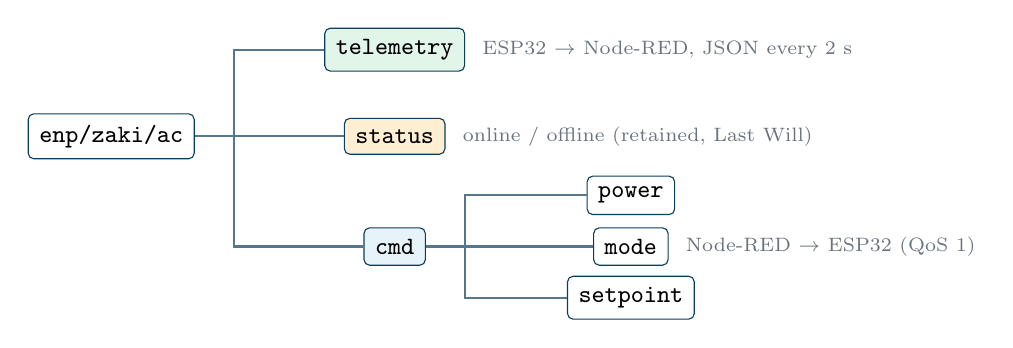
\begin{tikzpicture}[tn/.style={font=\small\ttfamily,draw=navy,rounded corners=2pt,fill=white,inner sep=4pt},
  e/.style={draw,thick,color=navy!70}]
  \node[tn] (root) at (0,0) {enp/zaki/ac};
  \node[tn,fill=okgreen!15] (tel) at (3.6,1.1) {telemetry};
  \node[tn,fill=amber!20] (sta) at (3.6,0) {status};
  \node[tn,fill=sky!10] (cmd) at (3.6,-1.4) {cmd};
  \node[tn] (pow) at (6.6,-0.75) {power};
  \node[tn] (mod) at (6.6,-1.4) {mode};
  \node[tn] (set) at (6.6,-2.05) {setpoint};
  \foreach \c in {tel,sta,cmd} \draw[e] (root.east) -- ++(0.5,0) |- (\c.west);
  \foreach \c in {pow,mod,set} \draw[e] (cmd.east) -- ++(0.5,0) |- (\c.west);
  \node[font=\scriptsize,color=codegray,anchor=west] at (tel.east) {\ ESP32 $\to$ Node-RED, JSON every 2 s};
  \node[font=\scriptsize,color=codegray,anchor=west] at (sta.east) {\ online / offline (retained, Last Will)};
  \node[font=\scriptsize,color=codegray,anchor=west] at (mod.east) {\ Node-RED $\to$ ESP32 (QoS 1)};
\end{tikzpicture}
\caption{MQTT topic hierarchy. Green: telemetry, amber: device status, blue: commands.}
\label{fig:topics}
\end{figure}

\begin{table}[H]
\centering\small
\caption{MQTT topics, publishers, subscribers and payloads.}
\label{tab:topics}
\begin{tabularx}{\linewidth}{@{}l l l c c X@{}}
\toprule
\textbf{Topic} & \textbf{Publisher} & \textbf{Subscriber} & \textbf{QoS} & \textbf{Retain} & \textbf{Payload} \\
\midrule
\topic{…/telemetry} & ESP32 & Node-RED & 0 & no & JSON, every \SI{2}{s} and after each command \\
\topic{…/status} & ESP32 / broker & Node-RED & 1 & yes & \texttt{online}; LWT \texttt{offline} \\
\topic{…/cmd/power} & Node-RED & ESP32 & 1 & no & \texttt{ON}, \texttt{OFF}, \texttt{TOGGLE} \\
\topic{…/cmd/mode} & Node-RED & ESP32 & 1 & no & \texttt{AUTO}, \texttt{COOL}, \texttt{HEAT}, \texttt{FAN} \\
\topic{…/cmd/setpoint} & Node-RED & ESP32 & 1 & no & number in [16, 30] \si{\celsius} \\
\bottomrule
\end{tabularx}
\end{table}

\noindent The ESP32 subscribes once to \topic{enp/zaki/ac/cmd/\#} and dispatches the message
according to the end of the topic. A telemetry message looks like:

\begin{lstlisting}[style=json]
{"temp":29.0,"hum":55.0,"setpoint":24.0,"power":"ON","mode":"AUTO","state":"COOLING","fan":3}
\end{lstlisting}

\subsection{Message sequences}
Figure~\ref{fig:sequence} details the three interactions of the system: connection with the
Last Will, periodic telemetry, and a remote command with its immediate acknowledgement through
a new telemetry message.

\begin{figure}[H]
\centering
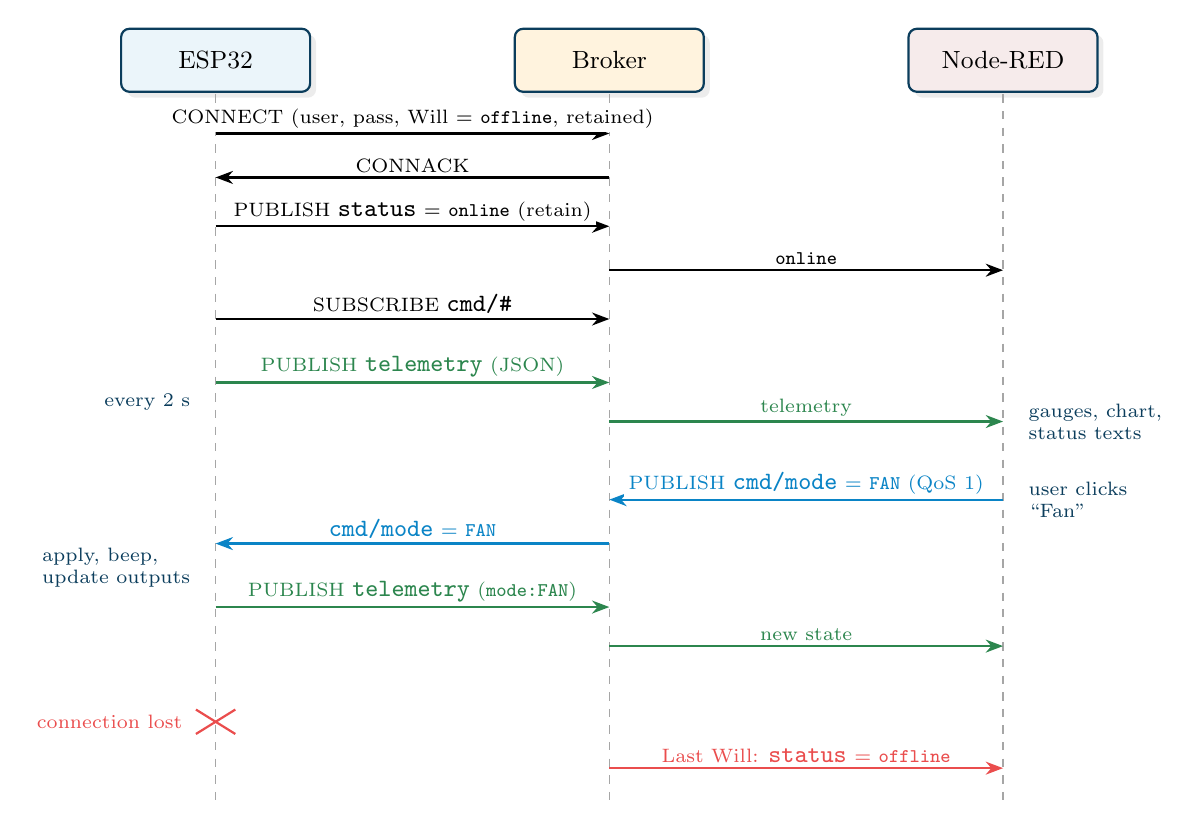
\begin{tikzpicture}[yscale=0.62,
  actor/.style={blk,minimum width=2.4cm,minimum height=0.8cm},
  msg/.style={-{Stealth[length=2.2mm]},thick},
  note/.style={font=\scriptsize,align=left,color=navy}]
  \node[actor,fill=sky!8] (E) at (0,0) {ESP32};
  \node[actor,fill=amber!15] (B) at (5,0) {Broker};
  \node[actor,fill=nrred!8] (N) at (10,0) {Node-RED};
  \foreach \x in {0,5,10} \draw[dashed,color=black!35] (\x,-0.7) -- (\x,-15.2);

  \draw[msg] (0,-1.5) -- node[lbl,above]{CONNECT (user, pass, Will = \texttt{offline}, retained)} (5,-1.5);
  \draw[msg] (5,-2.4) -- node[lbl,above]{CONNACK} (0,-2.4);
  \draw[msg] (0,-3.4) -- node[lbl,above]{PUBLISH \topic{status} = \texttt{online} (retain)} (5,-3.4);
  \draw[msg] (5,-4.3) -- node[lbl,above]{\texttt{online}} (10,-4.3);
  \draw[msg] (0,-5.3) -- node[lbl,above]{SUBSCRIBE \topic{cmd/\#}} (5,-5.3);

  \draw[msg,color=okgreen!70!black] (0,-6.6) -- node[lbl,above]{PUBLISH \topic{telemetry} (JSON)} (5,-6.6);
  \draw[msg,color=okgreen!70!black] (5,-7.4) -- node[lbl,above]{telemetry} (10,-7.4);
  \node[note,anchor=west] at (10.2,-7.4) {gauges, chart,\\status texts};
  \node[note,anchor=east] at (-0.2,-7.0) {every 2 s};

  \draw[msg,color=sky] (10,-9.0) -- node[lbl,above]{PUBLISH \topic{cmd/mode} = \texttt{FAN} (QoS 1)} (5,-9.0);
  \node[note,anchor=west] at (10.2,-9.0) {user clicks\\``Fan''};
  \draw[msg,color=sky] (5,-9.9) -- node[lbl,above]{\topic{cmd/mode} = \texttt{FAN}} (0,-9.9);
  \node[note,anchor=east] at (-0.2,-10.4) {apply, beep,\\update outputs};
  \draw[msg,color=okgreen!70!black] (0,-11.2) -- node[lbl,above]{PUBLISH \topic{telemetry} (\texttt{mode:FAN})} (5,-11.2);
  \draw[msg,color=okgreen!70!black] (5,-12.0) -- node[lbl,above]{new state} (10,-12.0);

  \draw[color=heatred,thick] (-0.25,-13.3) -- (0.25,-13.8) (-0.25,-13.8) -- (0.25,-13.3);
  \node[note,anchor=east,color=heatred] at (-0.3,-13.55) {connection lost};
  \draw[msg,color=heatred] (5,-14.5) -- node[lbl,above]{Last Will: \topic{status} = \texttt{offline}} (10,-14.5);
\end{tikzpicture}
\caption{Sequence diagram: connection and Last Will, telemetry, remote command, disconnection.}
\label{fig:sequence}
\end{figure}

\subsection{Choice of the broker and network constraint}
The first version used the public broker \texttt{broker.hivemq.com} on TCP port 1883. The
simulated ESP32 connected without problem, but the Node-RED server on the laptop stayed in the
``connecting'' state: the local network blocks outgoing traffic on non-web ports such as 1883,
8883. WebSocket tests from the same machine to several public brokers (ports 8000, 8081,
8084 and 8884) all timed out, while a WebSocket on port 443 opened immediately.

The final design therefore uses the free public broker \textbf{public.cloud.shiftr.io}
(credentials \texttt{public}/\texttt{public}), which accepts both transports at the same time:

\begin{itemize}
  \item the ESP32 connects with plain MQTT over TCP on port \textbf{1883} (PubSubClient library);
  \item Node-RED connects with MQTT over \textbf{secure WebSocket} on port \textbf{443}
        (URL \url{wss://public.cloud.shiftr.io}), which goes through the firewall like
        normal HTTPS traffic.
\end{itemize}

\noindent Both clients reach the same broker and the same topics, so the transport difference is
invisible to the application (Figure~\ref{fig:nr-config}). This illustrates a practical advantage of MQTT over WebSockets
in restricted networks.

\begin{figure}[H]
\centering
\begin{subfigure}[t]{0.47\linewidth}\centering
  \shot{fig/nodered_broker.png}
  \caption{Broker configuration: MQTT over WebSocket (\texttt{wss://}, port 443)}
\end{subfigure}\hfill
\begin{subfigure}[t]{0.47\linewidth}\centering
  \shot{fig/nodered_mqttin.png}
  \caption{\texttt{mqtt in} node: telemetry topic, QoS 0, parsed JSON output}
\end{subfigure}
\caption{MQTT configuration in Node-RED.}
\label{fig:nr-config}
\end{figure}

% ======================= 5. CONTROL LOGIC =========================
\section{Air-conditioning control logic}

\subsection{Operating modes}
\begin{itemize}
  \item \textbf{AUTO}: cools or heats as needed to reach the setpoint.
  \item \textbf{COOL}: cooling only. \quad \textbf{HEAT}: heating only.
  \item \textbf{FAN}: ventilation only, the compressor stays off.
  \item \textbf{OFF}: everything off and louver closed (from the dashboard or the local button).
\end{itemize}

\subsection{Thermostat with hysteresis}
A naive thermostat that switches at exactly the setpoint would turn the compressor on and off
at every small fluctuation of the measurement, which wears it out. A hysteresis band
$H = \SI{1}{\celsius}$ is used instead. With $T$ the measured temperature and $SP$ the setpoint:

\[
\text{cooling} \leftarrow
\begin{cases}
\text{ON}  & \text{if cooling is OFF and } T \ge SP + H\\
\text{OFF} & \text{if cooling is ON and } T \le SP\\
\text{unchanged} & \text{otherwise}
\end{cases}
\]
\[
\text{heating} \leftarrow
\begin{cases}
\text{ON}  & \text{if heating is OFF and } T \le SP - H\\
\text{OFF} & \text{if heating is ON and } T \ge SP\\
\text{unchanged} & \text{otherwise}
\end{cases}
\]


Figure~\ref{fig:hyst} illustrates the behaviour on a temperature profile: the compressor starts
only when the room exceeds \SI{25}{\celsius} and stops when it is back to \SI{24}{\celsius}.

\begin{figure}[H]
\centering
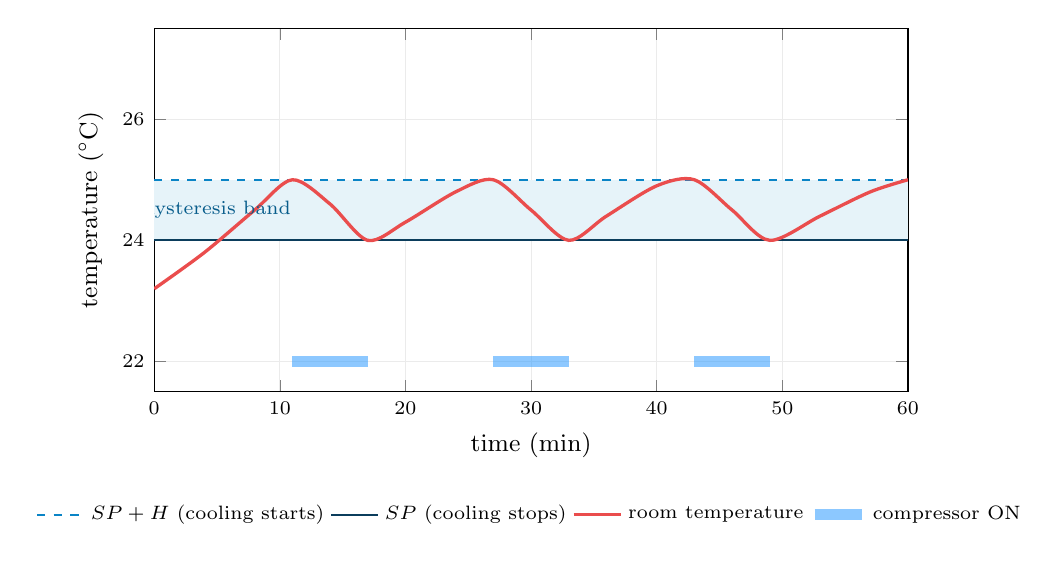
\begin{tikzpicture}
\begin{axis}[
  width=0.92\linewidth, height=6.2cm, xmin=0, xmax=60, ymin=21.5, ymax=27.5,
  xlabel={time (min)}, ylabel={temperature (\si{\celsius})},
  grid=major, grid style={black!8}, legend columns=4, legend style={font=\scriptsize,at={(0.5,-0.28)},anchor=north,draw=none},
  tick label style={font=\scriptsize}, label style={font=\small}]
  \fill[sky!10] (axis cs:0,24) rectangle (axis cs:60,25);
  \addplot[sky,dashed,thick,domain=0:60] {25}; \addlegendentry{$SP+H$ (cooling starts)}
  \addplot[navy,thick,domain=0:60] {24};       \addlegendentry{$SP$ (cooling stops)}
  \addplot[heatred,very thick,smooth] coordinates {
    (0,23.2) (4,23.8) (8,24.5) (11,25.0) (14,24.6) (17,24.0) (20,24.3) (24,24.8) (27,25.0)
    (30,24.5) (33,24.0) (36,24.4) (40,24.9) (43,25.0) (46,24.5) (49,24.0) (53,24.4) (57,24.8) (60,25.0)};
  \addlegendentry{room temperature}
  \addplot[coolblue,line width=4pt,opacity=0.55] coordinates {(11,22) (17,22)};
  \addplot[coolblue,line width=4pt,opacity=0.55,forget plot] coordinates {(27,22) (33,22)};
  \addplot[coolblue,line width=4pt,opacity=0.55,forget plot] coordinates {(43,22) (49,22)};
  \addlegendentry{compressor ON}
  \node[font=\scriptsize,color=sky!70!black] at (axis cs:5,24.5) {hysteresis band};
\end{axis}
\end{tikzpicture}
\caption{Illustration of the hysteresis control in cooling mode ($SP = \SI{24}{\celsius}$,
$H = \SI{1}{\celsius}$): few, long compressor cycles instead of rapid switching.}
\label{fig:hyst}
\end{figure}

\subsection{Fan speed and louver}
When the compressor runs, the fan speed depends on the gap $|T - SP|$
(Table~\ref{tab:fan}). The servo motor sweeps the louver between \ang{45} and \ang{135};
its angular step per \SI{20}{ms} equals the fan speed, so the swing is visibly faster at high
speed. When the unit is off, the louver closes at \ang{0}.

\begin{table}[H]
\centering\small
\caption{Fan speed selection.}
\label{tab:fan}
\begin{tabular}{@{}lll@{}}
\toprule
\textbf{Situation} & \textbf{Fan speed} & \textbf{Louver} \\
\midrule
Unit OFF & 0 (OFF) & closed (\ang{0}) \\
IDLE (setpoint reached) or $|T-SP| < \SI{2}{\celsius}$ & 1 (LOW) & slow swing \\
FAN mode, or $\SI{2}{\celsius} \le |T-SP| < \SI{5}{\celsius}$ & 2 (MEDIUM) & medium swing \\
$|T-SP| \ge \SI{5}{\celsius}$ & 3 (HIGH) & fast swing \\
\bottomrule
\end{tabular}
\end{table}

\subsection{State machine}
Figure~\ref{fig:fsm} summarises the states published in the \texttt{state} field of the
telemetry.

\begin{figure}[H]
\centering
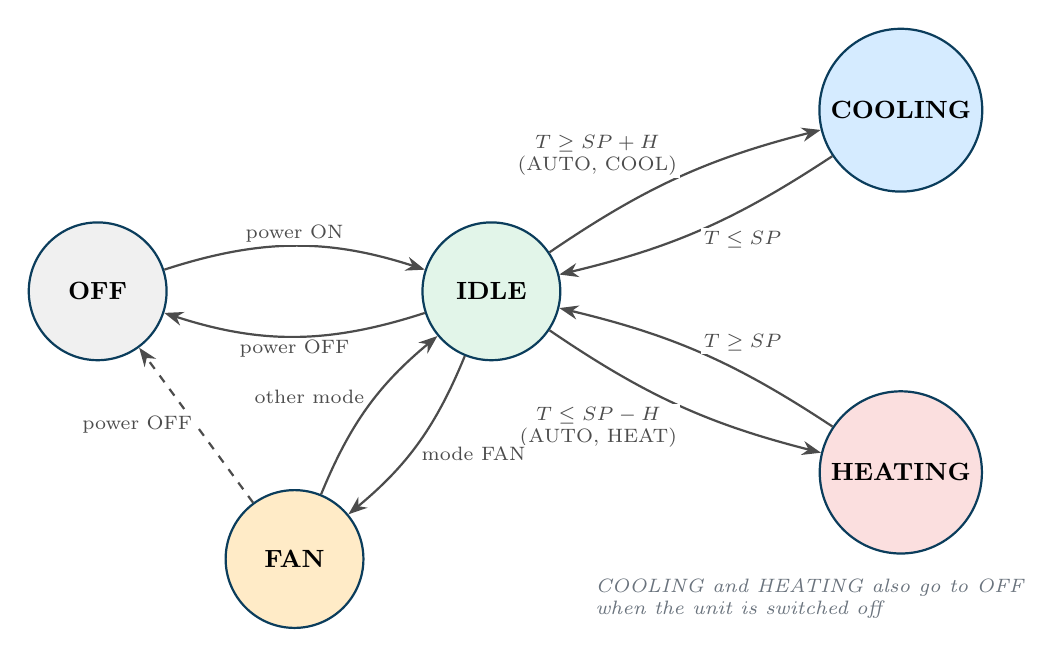
\begin{tikzpicture}[
  st/.style={circle,draw=navy,thick,minimum size=1.75cm,align=center,font=\small\bfseries},
  tr/.style={-{Stealth[length=2.4mm]},thick,color=black!70},
  tl/.style={font=\scriptsize,align=center,fill=white,inner sep=1pt}]
  \node[st,fill=black!6] (off) at (0,0) {OFF};
  \node[st,fill=okgreen!15] (idle) at (5,0) {IDLE};
  \node[st,fill=coolblue!20] (cool) at (10.2,2.3) {COOLING};
  \node[st,fill=heatred!18] (heat) at (10.2,-2.3) {HEATING};
  \node[st,fill=amber!25] (fan) at (2.5,-3.4) {FAN};

  \draw[tr] (off) to[bend left=18] node[tl,above]{power ON} (idle);
  \draw[tr] (idle) to[bend left=18] node[tl,below]{power OFF} (off);
  \draw[tr] (idle) to[bend left=10] node[tl,above left=-1pt]{$T \ge SP+H$\\(AUTO, COOL)} (cool);
  \draw[tr] (cool) to[bend left=10] node[tl,below right=-1pt]{$T \le SP$} (idle);
  \draw[tr] (idle) to[bend right=10] node[tl,below left=-1pt]{$T \le SP-H$\\(AUTO, HEAT)} (heat);
  \draw[tr] (heat) to[bend right=10] node[tl,above right=-1pt]{$T \ge SP$} (idle);
  \draw[tr] (idle) to[bend left=14] node[tl,below right]{mode FAN} (fan);
  \draw[tr] (fan) to[bend left=14] node[tl,above left]{other mode} (idle);
  \draw[tr,dashed] (fan) -- node[tl,left]{power OFF} (off);
  \node[font=\scriptsize\itshape,color=codegray,align=left,anchor=west] at (6.2,-3.9) {COOLING and HEATING also go to OFF\\when the unit is switched off};
\end{tikzpicture}

\caption{State machine of the air conditioner.}
\label{fig:fsm}
\end{figure}

% ======================= 6. FIRMWARE ==============================
\section{ESP32 firmware}

\subsection{Program structure}
The firmware is written in C++ with the Arduino framework and the libraries
\texttt{WiFi}, \texttt{PubSubClient} (MQTT client), \texttt{DHT sensor library},
\texttt{LiquidCrystal\_I2C} and \texttt{ESP32Servo}. The main loop is \textbf{non-blocking}: no
long \texttt{delay()}, so the MQTT connection, the button and the servo animation stay
responsive (Figure~\ref{fig:flowchart}).

\begin{figure}[H]
\centering
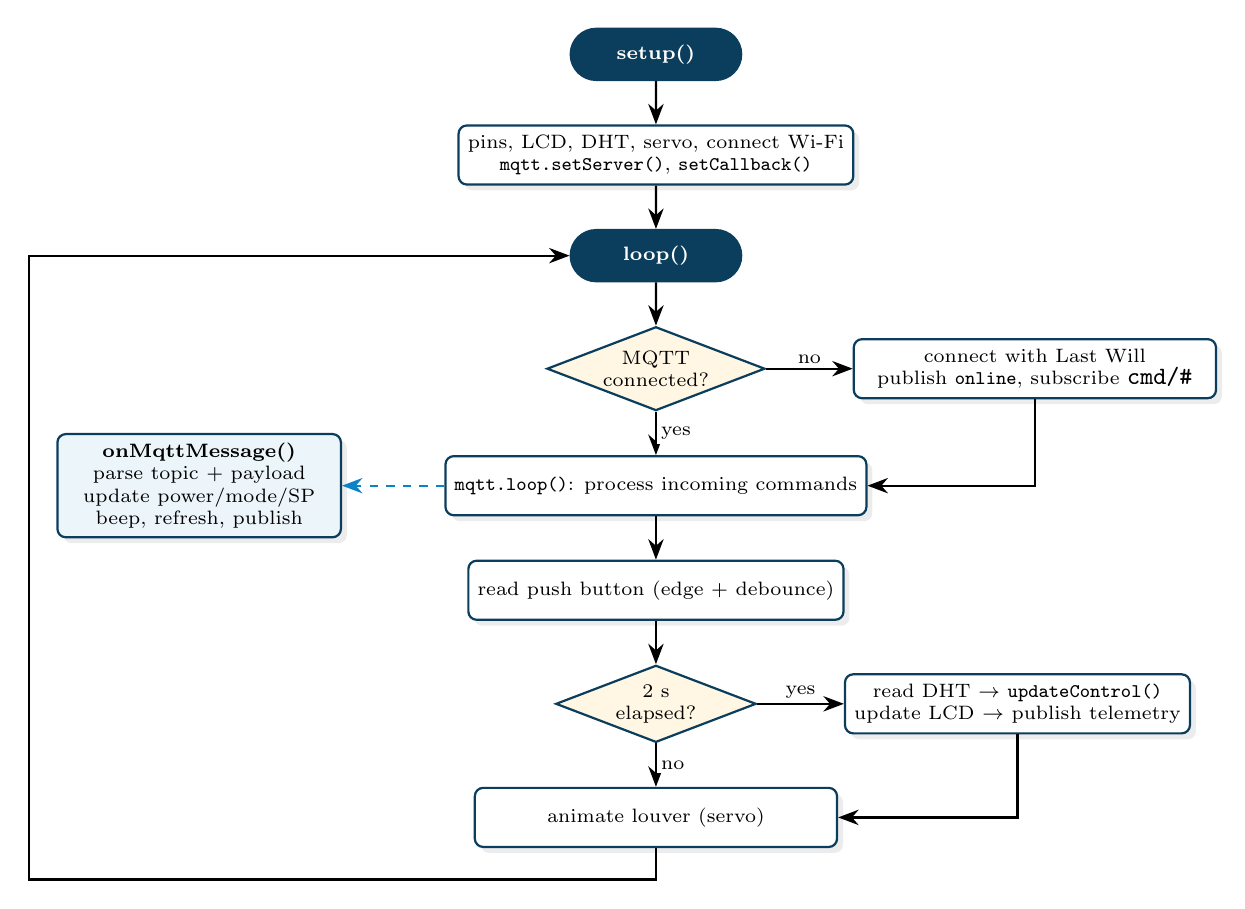
\begin{tikzpicture}[node distance=0.55cm,
  proc/.style={blk,minimum width=4.6cm,minimum height=0.75cm,font=\scriptsize},
  dec/.style={diamond,draw=navy,thick,aspect=2.6,inner sep=1pt,font=\scriptsize,align=center,fill=amber!12},
  term/.style={rounded rectangle,draw=navy,thick,fill=navy,text=white,font=\scriptsize\bfseries,minimum width=2.4cm,minimum height=0.65cm}]
  \node[term] (start) {setup()};
  \node[proc,below=of start] (init) {pins, LCD, DHT, servo, connect Wi-Fi\\\texttt{mqtt.setServer()}, \texttt{setCallback()}};
  \node[term,below=of init] (loop) {loop()};
  \node[dec,below=of loop] (con) {MQTT\\connected?};
  \node[proc,right=1.1cm of con] (rec) {connect with Last Will\\publish \texttt{online}, subscribe \topic{cmd/\#}};
  \node[proc,below=of con] (ml) {\texttt{mqtt.loop()}: process incoming commands};
  \node[proc,below=of ml] (btn) {read push button (edge + debounce)};
  \node[dec,below=of btn] (t2) {2 s\\elapsed?};
  \node[proc,right=1.1cm of t2,minimum width=4.2cm] (rd) {read DHT $\to$ \texttt{updateControl()}\\update LCD $\to$ publish telemetry};
  \node[proc,below=of t2] (sw) {animate louver (servo)};

  \node[proc,left=1.3cm of ml,minimum width=3.6cm,fill=sky!8] (cb) {\textbf{onMqttMessage()}\\parse topic + payload\\update power/mode/SP\\beep, refresh, publish};
  \draw[arr,dashed,color=sky] (ml.west) -- (cb.east);

  \draw[arr] (start) -- (init); \draw[arr] (init) -- (loop); \draw[arr] (loop) -- (con);
  \draw[arr] (con) -- node[lbl,above]{no} (rec);
  \draw[arr] (rec) |- (ml);
  \draw[arr] (con) -- node[lbl,right]{yes} (ml);
  \draw[arr] (ml) -- (btn); \draw[arr] (btn) -- (t2);
  \draw[arr] (t2) -- node[lbl,above]{yes} (rd);
  \draw[arr] (rd) |- (sw);
  \draw[arr] (t2) -- node[lbl,right]{no} (sw);
  \draw[arr] (sw.south) -- ++(0,-0.4) -| ($(cb.south west)+(-0.35,0)$) |- (loop.west);
\end{tikzpicture}
\caption{Flowchart of the firmware (setup, non-blocking main loop and MQTT callback).}
\label{fig:flowchart}
\end{figure}

\subsection{Key code excerpts}

\paragraph{Configuration.} Network, broker and topics are defined once at the top of the sketch.
\begin{lstlisting}[style=cpp]
const char* WIFI_SSID = "Wokwi-GUEST";            // Wokwi virtual access point
const char* MQTT_HOST = "public.cloud.shiftr.io"; // free public broker
const int   MQTT_PORT = 1883;
const char* MQTT_USER = "public";
const char* MQTT_PASS = "public";
#define BASE "enp/zaki/ac/"
const char* TOPIC_TELEMETRY = BASE "telemetry";
const char* TOPIC_STATUS    = BASE "status";
const char* TOPIC_CMD       = BASE "cmd/#";       // '#' = all command sub-topics
\end{lstlisting}

\paragraph{Connection with Last Will.} The connection is retried every \SI{3}{s} without
blocking. The Last Will is registered at connection time: retained message \texttt{offline} on
the status topic, with QoS 1.
\begin{lstlisting}[style=cpp]
void connectMqtt() {                       // non-blocking: 1 try every 3 s
  if (mqtt.connected() || millis() - lastMqttTry < 3000) return;
  lastMqttTry = millis();
  String id = "enp-ac-" + String((uint32_t)ESP.getEfuseMac(), HEX);
  // connect(id, user, pass, willTopic, willQos, willRetain, willMessage)
  if (mqtt.connect(id.c_str(), MQTT_USER, MQTT_PASS, TOPIC_STATUS, 1, true, "offline")) {
    mqtt.publish(TOPIC_STATUS, "online", true);  // retained
    mqtt.subscribe(TOPIC_CMD);
    publishTelemetry();
  }
}
\end{lstlisting}

\paragraph{Thermostat.} Direct translation of the equations of Section~5.2.
\begin{lstlisting}[style=cpp]
bool canCool = (mode == "COOL" || mode == "AUTO");
bool canHeat = (mode == "HEAT" || mode == "AUTO");
// Cooling: starts above SP + HYST, stops when SP is reached
if (!canCool)                                 cooling = false;
else if (!cooling && temp >= setpoint + HYST) cooling = true;
else if ( cooling && temp <= setpoint)        cooling = false;
// Heating: starts below SP - HYST, stops when SP is reached
if (!canHeat)                                 heating = false;
else if (!heating && temp <= setpoint - HYST) heating = true;
else if ( heating && temp >= setpoint)        heating = false;

float gap = fabs(temp - setpoint);
if (cooling || heating) fanSpeed = (gap < 2) ? 1 : (gap < 5 ? 2 : 3);
else                    fanSpeed = 1;          // ventilation only
\end{lstlisting}

\paragraph{Command callback.} Called by \texttt{mqtt.loop()} for every message received on
\topic{cmd/\#}. Invalid values are ignored (input validation).
\begin{lstlisting}[style=cpp]
void onMqttMessage(char* topic, byte* payload, unsigned int len) {
  String msg;
  for (unsigned int i = 0; i < len; i++) msg += (char)payload[i];
  msg.trim();
  String t = topic, up = msg; up.toUpperCase();
  if (t.endsWith("/power")) {
    if (up == "ON" || up == "TRUE" || up == "1")        power = true;
    else if (up == "OFF" || up == "FALSE" || up == "0") power = false;
    else if (up == "TOGGLE")                            power = !power;
  } else if (t.endsWith("/mode")) {
    if (up == "AUTO" || up == "COOL" || up == "HEAT" || up == "FAN") mode = up;
  } else if (t.endsWith("/setpoint")) {
    float v = msg.toFloat();
    if (v >= 16 && v <= 30) setpoint = v;         // reject out-of-range values
  } else return;
  beep();
  refreshAll();        // updateControl() + updateLcd() + publishTelemetry()
}
\end{lstlisting}

\paragraph{Telemetry.} The JSON payload is built with \texttt{snprintf} (no extra library).
\begin{lstlisting}[style=cpp]
void publishTelemetry() {
  if (!mqtt.connected() || isnan(temp)) return;   // nothing valid to send yet
  char json[200];
  snprintf(json, sizeof(json),
    "{\"temp\":%.1f,\"hum\":%.1f,\"setpoint\":%.1f,\"power\":\"%s\","
    "\"mode\":\"%s\",\"state\":\"%s\",\"fan\":%d}",
    temp, hum, setpoint, power ? "ON" : "OFF", mode.c_str(), state.c_str(), fanSpeed);
  mqtt.publish(TOPIC_TELEMETRY, json);
}
\end{lstlisting}

The complete source code is given in Appendix~\ref{app:code}.

% ======================= 7. NODE-RED ==============================
\section{Node-RED application}

\subsection{Flow}
The flow (Figure~\ref{fig:flow}) is organised in three parts, each one labelled with a comment
node:
\begin{enumerate}
  \item \textbf{Telemetry}: an \texttt{mqtt in} node subscribed to \topic{…/telemetry} with JSON
        parsing, a \texttt{debug} node, and a \texttt{function} node with nine outputs that
        splits the message for the widgets.
  \item \textbf{Commands}: the power switch, the mode button group and the setpoint slider are
        each wired to an \texttt{mqtt out} node publishing on the matching command topic with
        QoS 1.
  \item \textbf{Device status}: an \texttt{mqtt in} node on \topic{…/status} and a
        \texttt{change} node (JSONata) that turns \texttt{online}/\texttt{offline} into a
        coloured label.
\end{enumerate}

\begin{figure}[H]
\centering
\shot{fig/nodered_flow.png}
\caption{Node-RED flow. The green ``connected'' status under the MQTT nodes confirms the link
with the broker.}
\label{fig:flow}
\end{figure}

\begin{table}[H]
\centering\small
\caption{Main nodes of the flow.}
\label{tab:nodes}
\begin{tabularx}{\linewidth}{@{}>{\raggedright\arraybackslash}p{3.6cm} >{\raggedright\arraybackslash}p{3.0cm} X@{}}
\toprule
\textbf{Node} & \textbf{Type} & \textbf{Configuration / role} \\
\midrule
telemetry & mqtt in & \topic{enp/zaki/ac/telemetry}, QoS 0, output parsed JSON object \\
Parse telemetry & function & 9 outputs: temperature, humidity, chart, state, fan, power,
  mode, setpoint, alert \\
Temperature, Humidity & ui-gauge & half gauges with coloured segments (0--\SI{50}{\celsius}, 0--100\,\%) \\
History & ui-chart & line chart, two series (room temperature, setpoint), last 10 minutes \\
State, Fan, Device & ui-text & compressor state, fan speed, ESP32 online/offline \\
High temp alert & ui-notification & red pop-up when $T \ge \SI{35}{\celsius}$ \\
Power, Mode, Setpoint & ui-switch, ui-button-group, ui-slider & user controls,
  \texttt{passthru} disabled to avoid feedback loops \\
cmd/power, cmd/mode, cmd/setpoint & mqtt out & publish commands, QoS 1 \\
status (LWT), pretty status & mqtt in, change & retained status $\to$ ``ONLINE''/``OFFLINE'' \\
shiftr.io public broker & mqtt-broker & \texttt{wss://public.cloud.shiftr.io}, port 443 \\
\bottomrule
\end{tabularx}
\end{table}

\subsection{The ``Parse telemetry'' function}
Besides routing each field to its widget, the function performs two useful tasks:
\begin{itemize}
  \item \textbf{control synchronisation}: when the state changes on the device side (for example
        after a press on the local button), the switch, the mode buttons and the slider are
        updated. Messages are sent when the value changes (stored in the node context) and
        once every five messages, so that a freshly opened dashboard is synchronised too,
        while the slider does not jump back constantly while the user moves it;
  \item \textbf{alert on transition}: the overheating notification is sent once when the
        temperature crosses \SI{35}{\celsius}, not every two seconds.
\end{itemize}

\begin{lstlisting}[style=js]
const d = msg.payload;
if (typeof d !== 'object' || d === null) return null;
const last = context.get('last') || {};
const n = (context.get('n') || 0) + 1;  context.set('n', n);
const changed = (k) => { const c = last[k] !== d[k] || n % 5 === 0; last[k] = d[k]; return c; };
const out = [
  { payload: d.temp },                                       // 1 temperature gauge
  { payload: d.hum },                                        // 2 humidity gauge
  [ { topic: 'Room temperature', payload: d.temp },          // 3 chart (2 series)
    { topic: 'Setpoint', payload: d.setpoint } ],
  { payload: icons[d.state] || d.state },                    // 4 state text
  { payload: fanTxt },                                       // 5 fan text
  changed('power')    ? { payload: d.power }    : null,      // 6 sync power switch
  changed('mode')     ? { payload: d.mode }     : null,      // 7 sync mode buttons
  changed('setpoint') ? { payload: d.setpoint } : null,      // 8 sync slider
  null                                                       // 9 alert
];
const hot = d.temp >= 35;                                    // alert only on transition
if (hot && !context.get('hot')) out[8] = { payload: 'Room temperature is ' + d.temp + ' °C !' };
context.set('hot', hot);  context.set('last', last);
return out;
\end{lstlisting}

\subsection{Dashboard}
The dashboard (Figure~\ref{fig:dash}) is served by Node-RED at
\texttt{http://localhost:1880/dashboard/ac}. It is organised in four groups on a 12-column grid:
room climate (two gauges), remote control (power, mode, setpoint), status (ESP32 connection,
compressor state, fan speed) and history (chart of the temperature against the setpoint).

\begin{figure}[H]
\centering
\shot{fig/dashboard_main.png}
\caption{Node-RED dashboard during the test scenario (room at \SI{36}{\celsius}, cooling at
high fan speed). The chart shows the temperature history against the setpoint.}
\label{fig:dash}
\end{figure}

% ======================= 8. TESTS =================================
\section{Tests and results}

\subsection{Test procedure}
The tests were run with the real chain: Wokwi simulation in the browser, public broker
on the Internet, Node-RED on the laptop. The temperature was changed with the DHT slider of
Wokwi, the commands were sent from the dashboard, and every reaction was checked on three
sides: the simulated hardware (LEDs, LCD, servo), the serial monitor and the dashboard.

\begin{table}[H]
\centering\small
\caption{Test scenarios and observed results.}
\label{tab:tests}
\begin{tabularx}{\linewidth}{@{}c l X c@{}}
\toprule
\textbf{\#} & \textbf{Action} & \textbf{Observed result} & \textbf{Status} \\
\midrule
T1 & Start, $T=\SI{29}{\celsius}$, $SP=\SI{24}{\celsius}$, AUTO & blue LED on, state COOLING, fan HIGH (gap \SI{5}{\celsius}), dashboard ONLINE & \textcolor{okgreen}{\textbf{pass}} \\
T2 & Room cooled step by step to \SI{23.9}{\celsius} & fan HIGH $\to$ MEDIUM $\to$ LOW as the gap shrinks; compressor stops at \SI{23.9}{\celsius} (IDLE) and stays off up to \SI{24.4}{\celsius} (hysteresis) & \textcolor{okgreen}{\textbf{pass}} \\
T3 & Room at \SI{20.5}{\celsius}, then warming up & red LED on, HEATING, fan MEDIUM then LOW; heating stops at \SI{24.0}{\celsius} & \textcolor{okgreen}{\textbf{pass}} \\
T4 & Room at \SI{36.5}{\celsius} & COOLING, fan HIGH, red alert on the dashboard & \textcolor{okgreen}{\textbf{pass}} \\
T5 & Dashboard: mode FAN & \texttt{[SUB] cmd/mode <- FAN}, beep, compressor off, fan MEDIUM & \textcolor{okgreen}{\textbf{pass}} \\
T6 & Dashboard: setpoint \SI{30}{\celsius} at $T=\SI{29}{\celsius}$ & HEATING, fan LOW, LCD ``SP:30.0 HEATING'' & \textcolor{okgreen}{\textbf{pass}} \\
T7 & Dashboard: power OFF & all LEDs off, louver closed, LCD ``AC OFF'' & \textcolor{okgreen}{\textbf{pass}} \\
T8 & Stop the simulation & broker publishes the Last Will, dashboard shows OFFLINE & \textcolor{okgreen}{\textbf{pass}} \\
T9 & Short network interruption & \texttt{failed, rc=-2} then \texttt{OK}: automatic reconnection, telemetry resumes & \textcolor{okgreen}{\textbf{pass}} \\
\bottomrule
\end{tabularx}
\end{table}

\subsection{Screenshots}

\begin{figure}[H]
\centering
\begin{subfigure}{0.49\linewidth}\centering
  \shot{fig/wokwi_heating.png}
  \caption{T3: room at \SI{20.5}{\celsius}, HEATING (red LED)}
\end{subfigure}\hfill
\begin{subfigure}{0.49\linewidth}\centering
  \shot{fig/wokwi_fan.png}
  \caption{T5: FAN mode received from the dashboard}
\end{subfigure}\\[6pt]
\begin{subfigure}{0.49\linewidth}\centering
  \shot{fig/wokwi_off.png}
  \caption{T7: unit OFF, LEDs off, louver closed, ``AC OFF''}
\end{subfigure}
\caption{Wokwi circuit in the other states of the test scenario.}
\label{fig:wokwi-states}
\end{figure}

\noindent Listing~\ref{lst:serial} is an excerpt of the serial monitor recorded during the
scenario (identical consecutive lines removed). It shows every transition of Table~\ref{tab:tests},
including an automatic MQTT reconnection after a short network interruption (\texttt{rc=-2}).

\lstinputlisting[style=json,basicstyle=\ttfamily\scriptsize,caption={Serial monitor of the
ESP32 during the test scenario.},label={lst:serial},captionpos=b]{code/serial_log.txt}

\begin{figure}[H]
\centering
\shot{fig/dashboard_alert.png}
\caption{Dashboard: overheating alert ($T \ge \SI{35}{\celsius}$).}
\label{fig:dash-alert}
\end{figure}

\begin{figure}[H]
\centering
\shot{fig/dashboard_offline.png}
\caption{Dashboard after the simulation is stopped (T8): the Last Will marks the ESP32 as
OFFLINE. The history chart shows the whole scenario: cooling down to the setpoint, heating
from \SI{20.5}{\celsius}, overheating at \SI{36.5}{\celsius} and return to \SI{29}{\celsius}.}
\label{fig:dash-offline}
\end{figure}

\subsection{Discussion of the results}
\begin{itemize}
  \item \textbf{Responsiveness}: a command is applied by the ESP32 as soon as it is received and
        the new state is published immediately, without waiting for the next 2-second cycle.
        Note that Wokwi ran at about 25\,\% of real time on the laptop, so the simulated
        2-second period lasted about 7 seconds of wall-clock time.
  \item \textbf{Robustness}: the firmware reconnects automatically (Wi-Fi and MQTT), the loop
        never blocks, and out-of-range commands (for example a setpoint of \SI{50}{\celsius})
        are rejected.
  \item \textbf{Consistency}: the device is the single source of truth. The dashboard controls
        are re-synchronised from the telemetry, so the local button and the dashboard never
        disagree.
\end{itemize}

% ======================= 9. LIMITS ================================
\section{Limitations and improvements}
\begin{itemize}
  \item \textbf{Security}: the public broker has no access control; anyone who knows the topics
        can read the data or send commands. A real product needs a private broker, TLS
        (port 8883 or WSS) and one set of credentials per device, plus topic access lists.
  \item \textbf{Sensor}: the DHT11 is accurate to \SI{\pm 2}{\celsius} only, with a resolution of
        \SI{1}{\celsius}; a DHT22 or an SHT31 would allow a smaller hysteresis band.
  \item \textbf{Actuators}: LEDs stand for the compressor and the heater. A real unit would drive
        relays or an inverter, with a minimum off-time to protect the compressor.
  \item \textbf{Simulation}: the room temperature is set by hand; a thermal model of the room
        (the temperature decreasing while cooling) would make the simulation closed-loop.
  \item \textbf{Features}: history stored in a time-series database (InfluxDB), weekly schedule,
        energy estimation, and notifications on a phone.
\end{itemize}

% ======================= 10. CONCLUSION ===========================
\section{Conclusion}
A complete connected air conditioner was designed, simulated and tested. The ESP32 measures the
room climate with the DHT11, applies a thermostat with hysteresis, drives its actuators and
local display, and communicates through MQTT. Node-RED provides a clear dashboard for
monitoring and remote control, and the Last Will mechanism gives a reliable online/offline
indicator. The project also showed a real-world constraint: when a network blocks the standard
MQTT port, MQTT over secure WebSockets on port 443 keeps the system working without changing
the device or the application logic.

% ======================= APPENDIX =================================
\appendix
\section{How to run the project}
\begin{enumerate}
  \item Open the Wokwi project (\url{https://wokwi.com/projects/481300995020006401}) and press
        the green \emph{Start} button. The serial monitor shows \texttt{MQTT connecting... OK}.
  \item Start Node-RED (\texttt{start-node-red.bat} installs Node-RED and Dashboard 2.0 and
        imports \texttt{flows.json} on the first run).
  \item Open \texttt{http://localhost:1880/dashboard/ac}.
  \item Keep the Wokwi tab visible: browsers slow down hidden tabs, which slows the simulation.
  \item Click on the DHT sensor in Wokwi to change the temperature and humidity.
\end{enumerate}

\section{Complete firmware}
\label{app:code}
\lstinputlisting[style=cpp]{code/sketch.ino}

\end{document}
